\documentclass[12pt]{article}
\usepackage[margin=1in]{geometry} 		% defines page margin
\usepackage{knitting} 				% defines \chart and \textknit
\usepackage{titling} 				% title page
\usepackage{graphicx,xspace, scrextend}	% defines space control stuff
\usepackage{tabularx, array, colortbl}	% defines tables
\usepackage{multicol} 				% defines columns
\usepackage{multirow} 				% defines multirows, combined cells in tables
\usepackage{framed} 				% defines boxes for notes and written directions
\usepackage[x11names]{xcolor} 		% extends color library
\usepackage{hyperref}				% hyperlinks
\hypersetup{
    colorlinks=true,
    linkcolor=blue,
    filecolor=magenta,      
    urlcolor=blue,
}

\pdfmapfile{+knitfont.map}

\renewcommand{\arraystretch}{2}

\newcolumntype{L}[1]{>{\leftalign\arraybackslash}p{#1}}
\newcolumntype{C}[1]{>{\centering\arraybackslash}p{#1}}

% length parameters
\setlength{\parindent}{0pt} % disables indentation for paragraphs
\setlength{\columnsep}{0.7cm} % column separation in multicol environment

% color parameters
\colorlet{framecolor}{black}
\colorlet{shadecolor}{LemonChiffon1}
\colorlet{highlight}{yellow}

% custom commands
\newcommand{\comment}[1]{} % allows for multiline comments that LaTeX will ignore

\newcommand{\vocab}[1]{\emph{\textbf{#1}}} % format for highlighting definitions of stitches, vocabulary terms
\newcommand{\rowDir}[1]{\textbf{#1:}} % indent for written instructions within paragraphs

\renewcommand{\repeat}[1]{\textbf{*[#1]*}} % format for written repeats, bold with *[ stitches ]*

\newcommand{\increase}[1]{(\emph{+#1 
	\ifnum#1=1{st}\else{sts}\fi})}
\newcommand{\decrease}[1]{(\emph{$-$#1
	\ifnum#1=1{st}\else{sts}\fi})}
\newcommand{\stitchcount}[1]{(\emph{#1 sts})}

\renewcommand{\rm}{\vocab{rm}} % remove marker
\renewcommand{\pm}{\vocab{pm}} % place marker

% thick horizontal line
\makeatletter \newcommand{\thickhline}{
    \noalign {\ifnum 0=`}\fi \hrule height 1.5pt
    \futurelet \reserved@a \@xhline
}
\makeatother

% custom environments
\newenvironment{frnote}
    {% framed environment for pattern notes
    	\setlength{\FrameRule}{1.5pt}
    	\def\FrameCommand{\fboxrule=\FrameRule\fboxsep=\FrameSep \fcolorbox{framecolor}{shadecolor}}
    	\MakeFramed {\FrameRestore}}
    {\setlength{\FrameRule}{1pt}
	\endMakeFramed}

\newenvironment{frdirection}
    {% framed environment for written directions
	\def\FrameCommand{\fboxrule=\FrameRule\fboxsep=\FrameSep \fbox}
   	\MakeFramed {\advance\hsize-\width \FrameRestore}
    	\addmargin[1.5cm]{0pt}}
    {\endaddmargin
	\endMakeFramed}

\newenvironment{unframed}
    {% unframed environment for written directions
	\setlength{\parindent}{-2em}
	\begin{addmargin}[2em]{0pt}}
    {\end{addmargin}
	\setlength{\parindent}{0em}}

\title{Sandbloom}
\author{Shanel Wu (Piper Nell)}

\begin{document}
\begin{titlingpage}

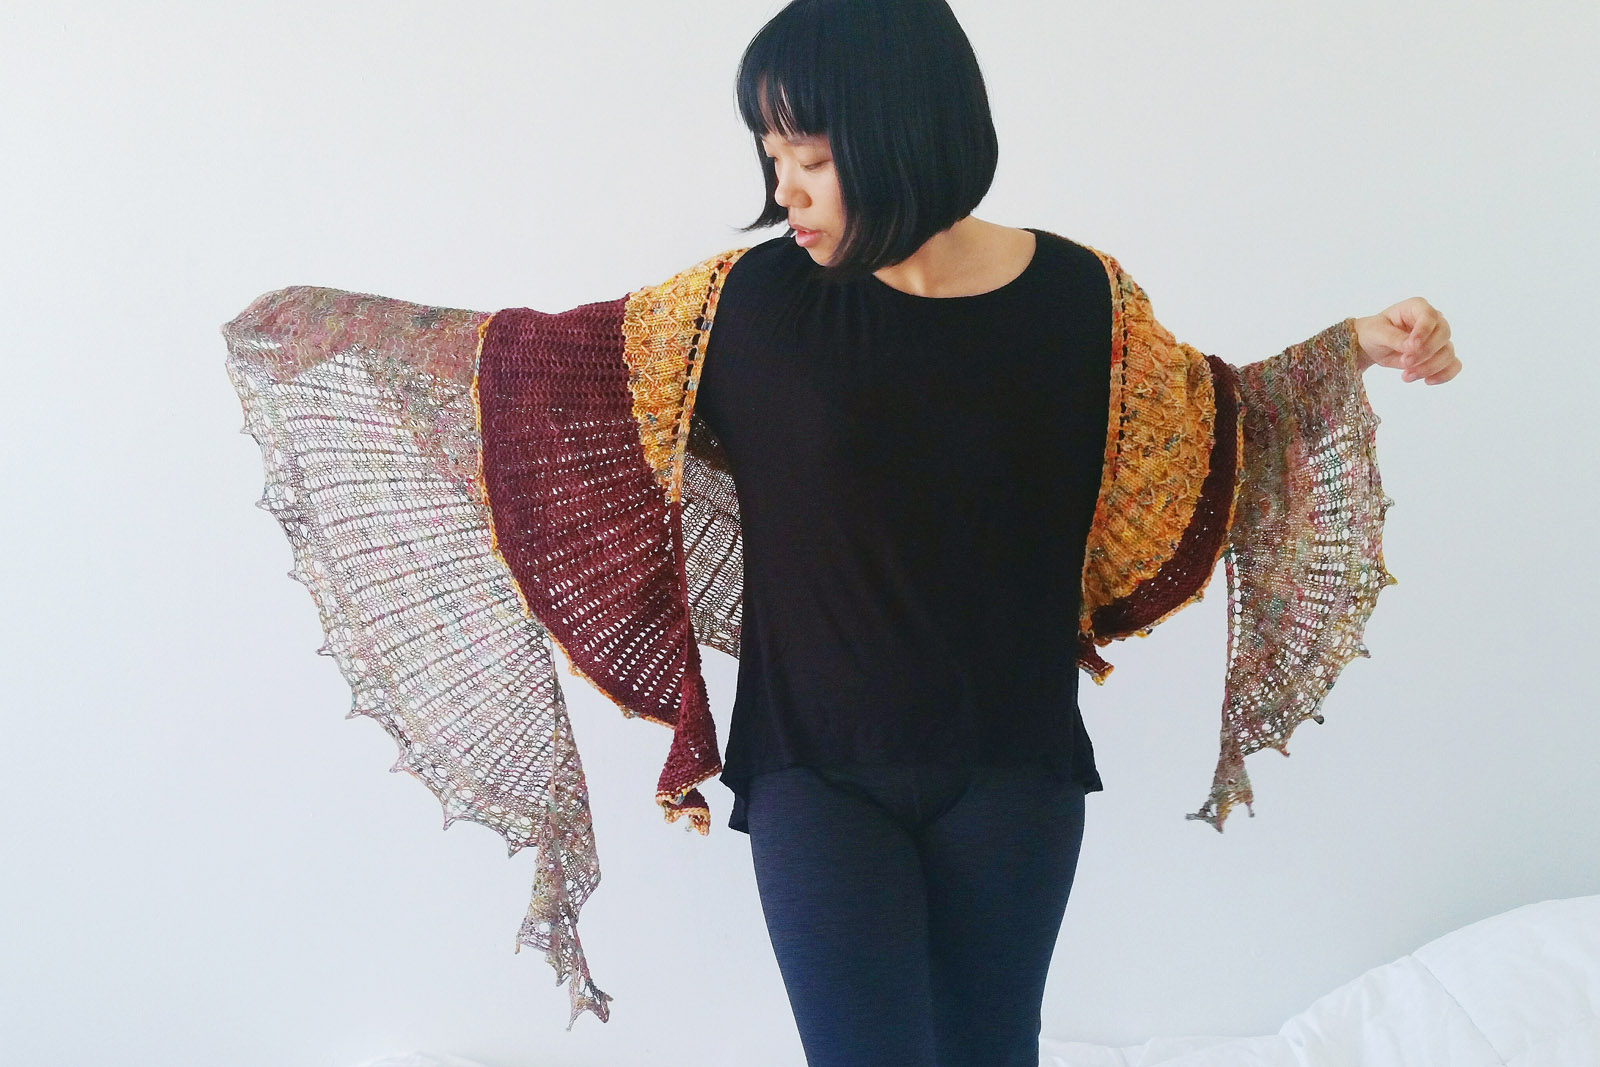
\includegraphics[width=6.5in]{both-arms.jpg}

\begin{multicols}{2}

\section*{\thetitle}
\subsubsection*{\theauthor}

Have you ever seen a desert in bloom? Many people think of a barren, punishing land when they think of a ``desert". Yet in my native Mojave Desert surrounding Las Vegas, the landscape comes alive after a rainstorm. This shawl is inspired by various flowering plants in the Mojave. The textured stitch patterns evoke barrel cacti, sagebrush branches, and prickly pears while the shape mimics the asymmetrical, yet beautiful, way that many plants propagate.

\vspace{-1em}
\subsubsection*{Materials}

For this shawl, you'll need two 100g skeins of yarn and a long (at least 40") circular needle. Choose your weight \textbf{[fingering or DK]} and color option \textbf{[one or two colors]}. If you tend to bind off tightly, you may want an additional needle 2 or 3 sizes larger. \\ 
\textbf{Fingering Weight:} 2 100g/437y skeins, \emph{(rec: Krityum Handmade - Rozaana or Jhilmil)}, needle: US5/3.75mm \\
\textbf{DK Weight:} 2 100g/225y skeins, \emph{(rec: Krityum Handmade - Cozy Sweater Light)}, needle: US7/4.5mm \\ Gauge is not important, but may affect yarn consumption and final size of the piece.

\vspace{-1em}
\subsubsection*{Notions}
\vspace{-0.7em}
\begin{itemize}
\item Tapestry needle \vspace{-1em}
\item Removable stitch markers
\end{itemize}

\vspace{-2em}

\subsubsection*{Reading/Techniques}

This shawl is recommended for advanced beginners who are familiar with yo, k2tog, and ssk sts; picking up sts; and slipping sts.

\vspace{.5em}
One set of directions is given for both versions of the shawl, fingering weight and DK weight. Repeat and stitch counts differ by yarn weight and are given in the format \mbox{\vocab{fingering (DK)}. [e.g. knit 45(35) sts]} 

\end{multicols}

\end{titlingpage}

\newpage

%%%%%%%%%%%%%%%%%%%%%%%%%%%%%%%%%%%%%%%%
\subsection*{Pattern Key}

Pattern repeats will be indicated with thick borders (chart) or \textbf{*[stitches]*} (written). 
\vspace{-1em}
\begin{center}
\begin{tabular}{| C{0.15\linewidth}  C{0.2\linewidth}  p{0.6\linewidth} | }
\thickhline \rowcolor{shadecolor} 
\textbf{Chart}	& \textbf{Written}	& \textbf{Name \& Description} \\ \thickhline
\chart{-}	& k (RS); p (WS)	&  knit (RS); purl (WS)	\\
\chart{=} 	& p (RS); k (WS)	& purl  (RS); knit (WS) \\
\chart{6}		& s1 wyif		& slip one stitch purlwise with yarn in front \\
\chart{h}	& k uls		& \textbf{knit under loose strand:} insert needle front to back under loose strand, then into next stitch knitwise. Knit stitch normally and bring new stitch under strand from back to front. \emph{(See appendix for picture tutorial.)}\\
\chart{S}	& pm		& place marker (after stitch) \\
\chart{""}	& w\&t 	& \textbf{wrap \& turn:} \emph{See Section 2, Sagebrush Lace}\\
\multicolumn{3}{| c |}{\cellcolor{shadecolor}\textbf{increases}} \\ 
\chart{O} 	& yo		& yarn-over  \\
\chart{Z}	& w3k		& \textbf{wrap 3 knit:} insert needle into stitch knitwise, wrap yarn three times and pull all three loops through; worked as a single stitch on next row \\
\chart{w}	& kyok	& \textbf{knit yarn-over knit:} in a single stitch, knit, yarn over, then knit again; double increase		\\ 
\multicolumn{3}{| c |}{\cellcolor{shadecolor} \textbf{decreases}} \\ \
\chart{>}	& k2tog 	& \textbf{knit 2 together:} single decrease, right-leaning \\
\chart{<}	& ssk		& \textbf{slip slip knit:} single decrease, left-leaning \\
\chart{A} 	& cdd		& \textbf{central double-decrease:} slip two stitches as if to k2tog, k next stitch, pass 2 slipped st over \\
\chart{R}	& k3tog 	& \textbf{knit 3 together:} double decrease, right-leaning \\
\chart{L}	& sssk		& \textbf{slip slip slip knit:} slip 3 knitwise individually, k3tog through back loop; double decrease, left-leaning \\
\hline
\end{tabular}
\end{center}

\newpage

\begin{multicols}{2}
\section*{Cast On and Set Up}
Work garter tab cast on, then work \textbf{Chart A} once.
\vspace{-1em}
\subsubsection*{Garter Tab Cast On}

\begin{enumerate}
\item CO 3 sts using the long-tail method. Knit 6 rows in garter stitch. \stitchcount{3}
\item After the last row, do not turn work and instead, rotate work by 90 degrees clockwise. Pick up and knit 3 stitches into the garter edge. \stitchcount{6}
\item Rotate work 90 degrees clockwise again. Pick up and knit 3 stitches along the cast on edge. \stitchcount{9}
\end{enumerate}

\subsection*{Chart A (written)}

\begin{unframed}
\hspace{-2em}\rowDir{Row 1} k3, yo, k3, yo, k3 \stitchcount{11}

\rowDir{Row 2} k3, kyok, p3, kyok, k3 \stitchcount{15}

\rowDir{Row 3} k3, yo, k1, p2, k3, p2, k1, yo, k3 \stitchcount{17}

\rowDir{Row 4} k3, kyok, p1, k2, p3, k2, p1, kyok, k3 \stitchcount{21}
\end{unframed}

\vfill
\begin{center}
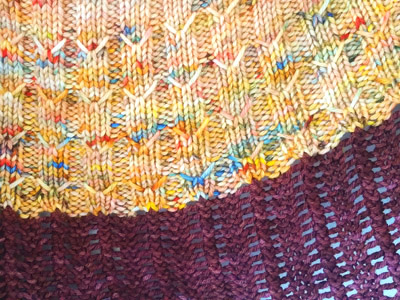
\includegraphics[width=3in]{detail1.jpg}
\end{center}
\vfill
\columnbreak

\section*{S1: Cactus Rib}

This section is comprised of a rib-based slip stitch texture that grows with the crescent shaping. Work 10 (6) repeats of the Cactus Rib stitch \textbf{(Chart B)}. Each 10-row repeat increases the total stitch count by 30 sts.

\begin{frnote}
\textbf{Tip:} when working \textbf{sl3 wyif}, keep the working yarn \emph{loose} for the loose strand.
\end{frnote}

\subsection*{Chart B (written)}
\begin{unframed}
\hspace{-2em}\rowDir{Row 1} (RS) k3, yo, p1, \repeat{k3, p2} to last 7 sts, k3, p1, yo, k3

\rowDir{Row 2} (WS) k3, kyok, k1, p3, \repeat{k2, p3} to last 5 sts, k1, kyok, k3

\rowDir{Row 3} k3, yo, k2, p2, \repeat{sl3 wyif, p2} to last 5 sts, k2, yo, k3

\rowDir{Row 4} k3, kyok, p2, \repeat{k2, p3} to last 8 sts, k2, p2, kyok, k3

\rowDir{Row 5} k3, yo, p2, \repeat{k3, p2} to last 3 sts, yo, k3

\rowDir{Row 6} k3, kyok, \repeat{k2, p3} to last 6 sts, k2, kyok, k3

\rowDir{Row 7} k3, yo, k3, p2, k3, p2, \repeat{k1, k uls, k1, p2} to last 11 sts, k3, p2, k3, yo, k3

\rowDir{Row 8} k3, kyok, p3, \repeat{k2, p3} to last 9 sts, k2, p3, kyok, k3

\rowDir{Row 9} k3, yo, k1, p2, \repeat{k3, p2} to last 4 sts, k1, yo, k3

\rowDir{Row 10} k3, kyok, p1, \repeat{k2, p3} to last 7 sts, k2, p1, kyok, k3
\end{unframed}

\vspace{1em}
At the end of Section 1, you should have 321 (201) sts.


\end{multicols}
\subsection*{Chart A: Set Up}

\chart{
\rnleft===W-==---==-W===
---O-==---==-O---\rnright
~~~\rnleft===W---W===
~~~---O---O---\rnright
}


\newpage

\subsection*{Chart B: Cactus Rib}
\chart{
~~~~~~~\rnleft===W-\!\overline{==---}\!==-W===
~~~~~~~---O-\!==---\!==-O---\rnright
~~~~~\rnleft===W---\!==---\!==---W===
---O---==---\!==-h-\!==---==---O---\rnright
~~~~~~~~\rnleft===W\!==---\!==W===
~~~~~~~~---O\!==---\!==O---\rnright
~~~~~~\rnleft===W--\!==---\!==--W===
~~~~~~---O--\!==666\!==--O---\rnright
~~~~\rnleft===W=---\!==---\!=W===
~~~~---O=---\!\underline{==---}\!=O---\rnright
}

\vspace{-1.2in}
\hspace{5.5in} 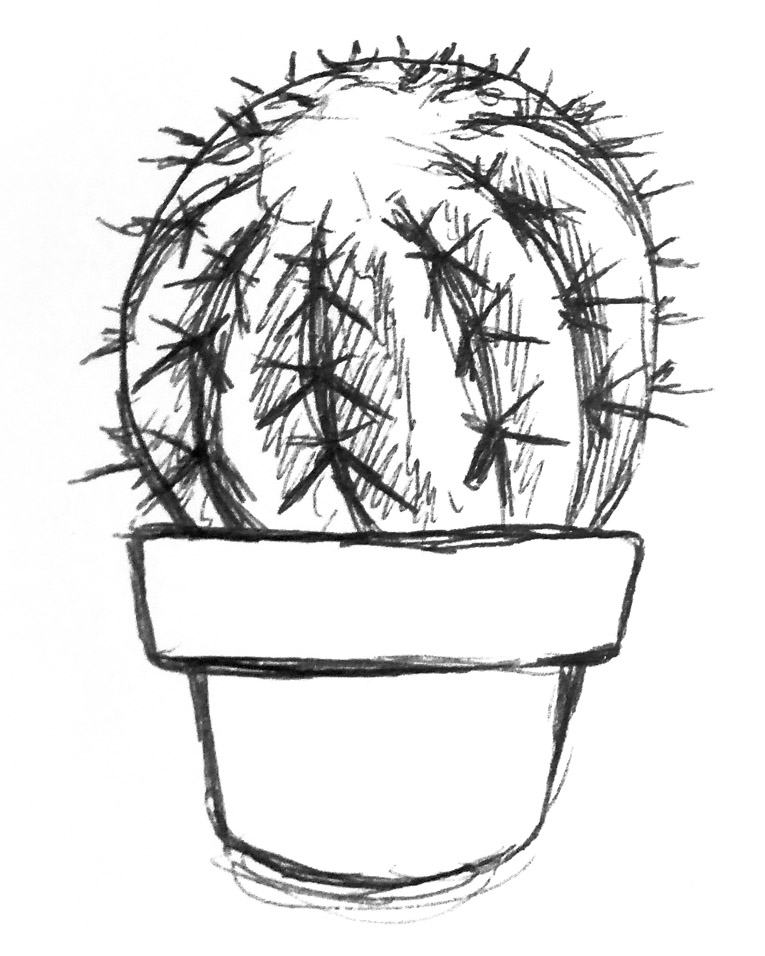
\includegraphics[height=1.7in]{1_barrel.jpg}

\vspace{-.4em}
\hspace{5.7in} \mbox{\emph{barrel cactus}}


\begin{multicols}{2}
\section*{S2: Sagebrush Lace}

\begin{frnote}
\textbf{2-color version:} break MC and switch to CC before beginning Section 2.
\end{frnote}

In this section, you will switch to a Shetland-inspired mesh stitch. Short rows will shape the shawl into an asymmetrical crescent. Note that odd and even rows have been switched so that \vocab{RS rows are even-numbered} on the chart.

\begin{frnote}
\rowDir{w\&t stitch} sl1 wyib, bring yarn to front, sl1 back to left needle to "wrap" stitch, turn. Chart: \chart{""}
\end{frnote}

Work set up rows \increase{6}, then work 6 (4) repeats of the Sagebrush Lace stitch \textbf{(Chart C)}. Each 10-row repeat increases the total stitch count by 15 sts.

\begin{unframed}
\hspace{-2em}\rowDir{Set Up 1} (RS) k3, yo, \repeat{k1, yo, cdd, yo, k1} to last 3 sts, yo, k3 \increase{2}

\rowDir{Set Up 2} (WS) k3, kyok, k to last 9 sts, w\&t \increase{2}

\rowDir{Set Up 3} (RS) \repeat{k1, yo, cdd, yo, k1} twice, \pm, \repeat{k1, yo, cdd, yo, k1} to last 6 sts, k3, yo, k3 \increase{1}
\end{unframed}

\subsection*{Chart C (written)}
\begin{unframed}
\hspace{-2em}\rowDir{Row 1} (WS) k3, kyok, k to marker, \rm \vocab{(remove marker)}, w\&t \emph{(All WS rows are identical to Row 1)}

\rowDir{Row 2} (RS) \repeat{k1, yo, cdd, yo, k1} twice, \pm, \repeat{k1, yo, cdd, yo, k1} to last 4 sts, k1, yo, k3

\rowDir{Row 4}  \repeat{k1, yo, cdd, yo, k1} twice, \pm, \repeat{k1, yo, cdd, yo, k1} to last 7 sts, k4, yo, k3

\rowDir{Row 6}  \repeat{k1, yo, cdd, yo, k1} twice, \pm, \repeat{k1, yo, cdd, yo, k1} to last 5 sts, k2, yo, k3

\rowDir{Row 8}  \repeat{k1, yo, cdd, yo, k1} twice, \pm, \repeat{k1, yo, cdd, yo, k1} to last 3 sts, yo, k3

\rowDir{Row 10}  \repeat{k1, yo, cdd, yo, k1} twice, \pm, \repeat{k1, yo, cdd, yo, k1} to last 6 sts, k3, yo, k3
\end{unframed}

After the last repeat of \textbf{Chart C}, you should have 417 (267) sts. On the next WS row, k3, kyok, then k across to last 4 sts, removing marker as you come to it. At every wrapped stitch, insert R needle knitwise into wrap, then knit the wrap and the stitch together. To finish the row, kyok and k last 3 sts. At the end of Section 2, you should have 421 (271) sts.
\end{multicols}

\subsection*{Chart C: Sagebrush Lace}
\chart{
~---O---\!\overline{-OAO-}\!SOAO--OAO-\rnright
~\rnleft===W===\!=====\!""
~~~~---O\!-OAO-\!SOAO--OAO-\rnright
~~~~\rnleft===W\!=====\!""
~~---O--\!-OAO-\!SOAO--OAO-\rnright
~~\rnleft===W==\!=====\!""
---O----\!-OAO-\!SOAO--OAO-\rnright
\rnleft===W====\!=====\!""
~~~---O-\!-OAO-\!SOAO--OAO-\rnright
~~~\rnleft===W=\!\underline{=====}\!""
}
 
\vspace{-2.6in}\hspace{5.2in}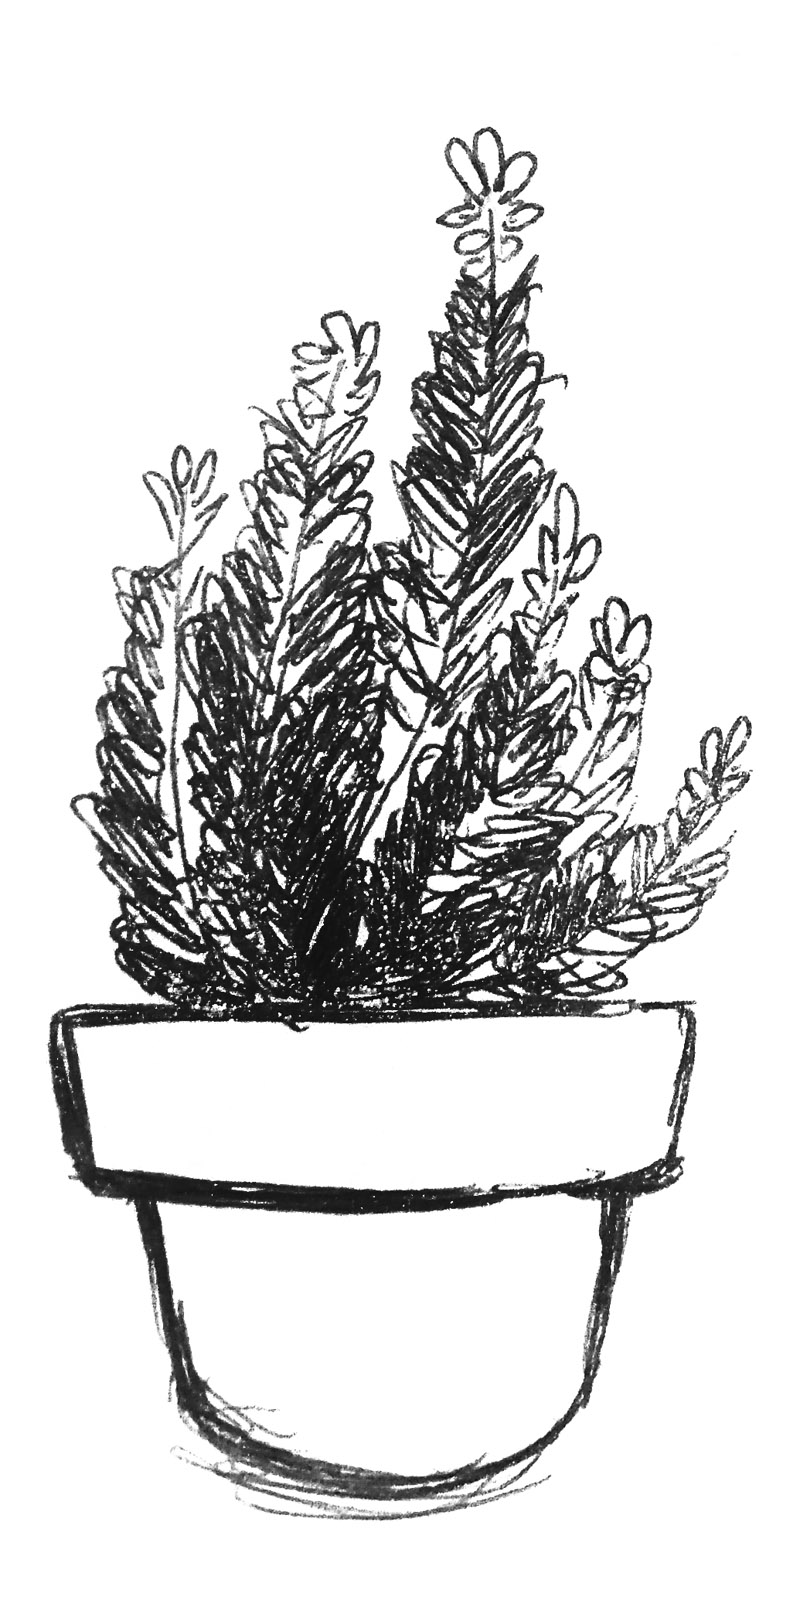
\includegraphics[height=2.9in]{2_sagebrush.jpg}

\vspace{-.6em}
\hspace{5.5in} \emph{sagebrush}

\vfill

\begin{multicols}{2}

\section*{S3: Prickly Pear Edge}

Work the following two rows 3 times, to create 3 garter ridges. \increase{18}
\begin{unframed}
\hspace{-2em}\rowDir{Row 1} (RS) k3, yo, k to last 3 sts, yo, k3

\rowDir{Row 2} (WS) k3, kyok, k to last 4 sts, kyok, k3
\end{unframed}

\begin{frnote}
\textbf{DK weight version:} Skip Chart D and proceed to bind off.
\end{frnote}

Work the Prickly Pear edge (\textbf{Chart D}) once. \increase{30}

\vfill

\subsection*{Chart D (written)}
\begin{unframed}
\hspace{-2em}\rowDir{Row 1} (RS) k3, yo, \repeat{k2, w3k, k2} to last 3 sts, yo, k3

\rowDir{Row 2} (WS) k3, kyok, \repeat{k2, kyok, k2} to last 4 sts, kyok, k3

\rowDir{Row 3} k3, yo, k3, \repeat{k3tog, yo, k1, yo, sssk} to last 6 sts, k3, yo, k3

\rowDir{Row 4} k3, kyok, k to last 4 sts, kyok, k3

\rowDir{Row 5} k3, yo, k to last 3 sts, yo, k3

\rowDir{Row 6} Repeat Row 4.

\rowDir{Row 7} k3, yo, k4, \repeat{k2tog, yo, k1, yo, ssk} to last 7 sts, k4, yo, k3

\rowDir{Row 8} Repeat Row 4.

\rowDir{Row 9} k3, yo, k2, \repeat{k2tog, yyo, k1, yo, ssk} to last 5 sts, k2, yo, k3

\rowDir{Row 10} Repeat Row 4.
\end{unframed}

\end{multicols}

\subsection*{Chart D: Prickly Pear Edge}
\chart{
~~\rnleft===W==\!\overline{=====}\!==W===
~~---O--\!<O-O>\!--O--- \rnright
\rnleft===W====\!=====\!====W===
---O----\!<O-O>\!----O--- \rnright
~~~\rnleft===W=\!=====\!=W===
~~~---O-\!-----\!-O--- \rnright
~\rnleft===W===\!=====\!===W===
~---O---\!LO-OR\!---O--- \rnright
~~~~\rnleft===W\!==W==\!W===
~~~~---O\!\underline{--Z--}\!O--- \rnright
}

\vspace{-2.5in} \hspace{5in}
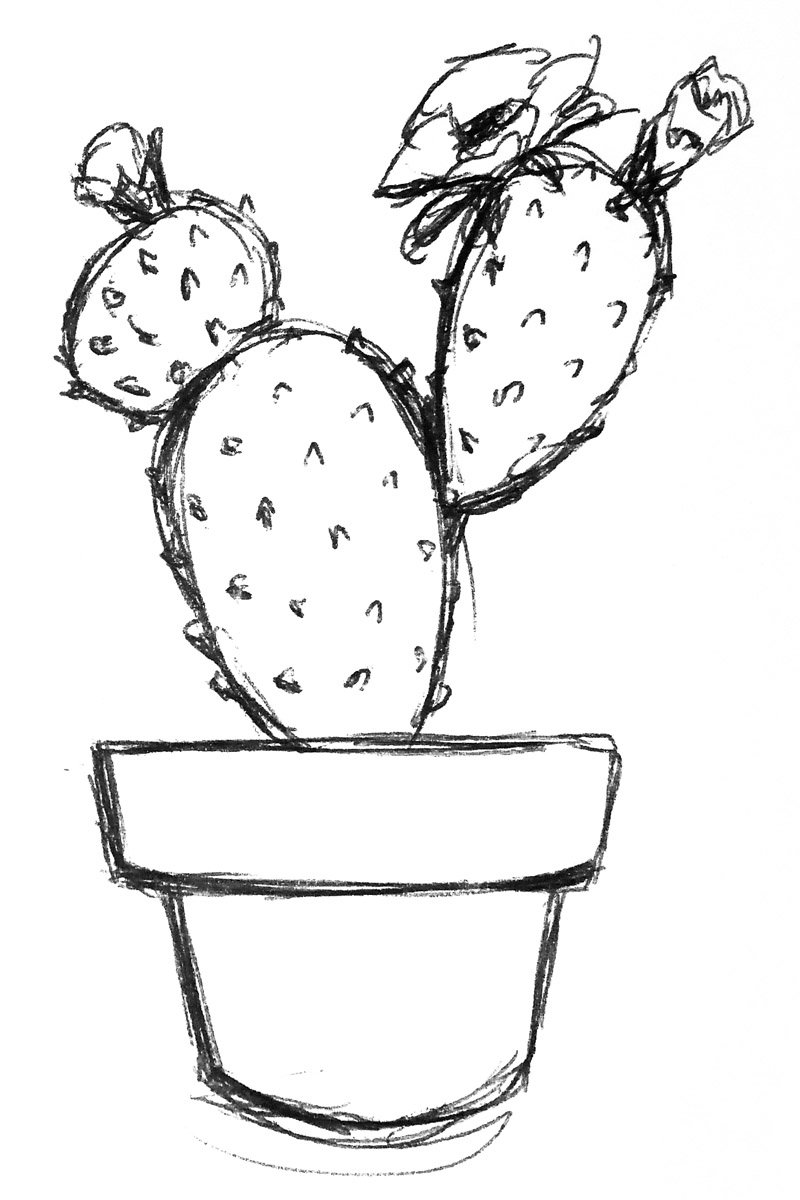
\includegraphics[height=2.3in]{3_pricklypear.jpg}

\vspace{-.5em}
\hspace{5.3in} \mbox{\emph{prickly pear}}

\newpage

\begin{multicols}{2}
\subsection*{Bind Off}
\begin{frnote}
\textbf{2-color version:} Break CC and switch back to MC for contrasting BO.
\end{frnote}

Before binding off, you should have 459 (319) sts. If you tend to bind off tightly, use the larger needle. You'll need:
\begin{enumerate}
\item \href{https://www.purlsoho.com/create/cable-cast-on/}{\underline{Cable Cast On} (CCO)}
\vspace{-0.5em}
\item \href{http://www.knitty.com/ISSUEfall09/FEATjssbo.php}{\underline{Jeny's Surprisingly Stretchy Bind Off} (JSSBO)}
\end{enumerate}

\begin{unframed}
\hspace{-2em}\rowDir{Row 1} (RS) k across

\rowDir{Row 2} (WS) CO 2 sts with CCO, BO 7 sts with JSSBO, \repeat{CCO 2 sts, JSSBO 12 sts} to last 7 sts, CCO 2 sts, JSSBO 6 sts, CCO 2  sts, JSSBO to end.
\end{unframed}

\vspace{1em}

Cut yarn, leaving a 6 inch tail, and pull end through last stitch. Weave in ends with your tapestry needle. 

\vspace{1em}
Block shawl into a crescent shape. The garter tab may create a ``peak" in the fabric before blocking, but the peak will block out. If you block aggressively, the lace in Sections 2 and 3 will open dramatically. If you block more moderately, the texture in Section 1 will retain more of its squish factor (recommended for DK weight version).

\subsection*{Appendix: \emph{k uls} stitch}

The \textbf{k uls} (knit under loose strand) cinches the loose strand behind a stitch.

\begin{center}
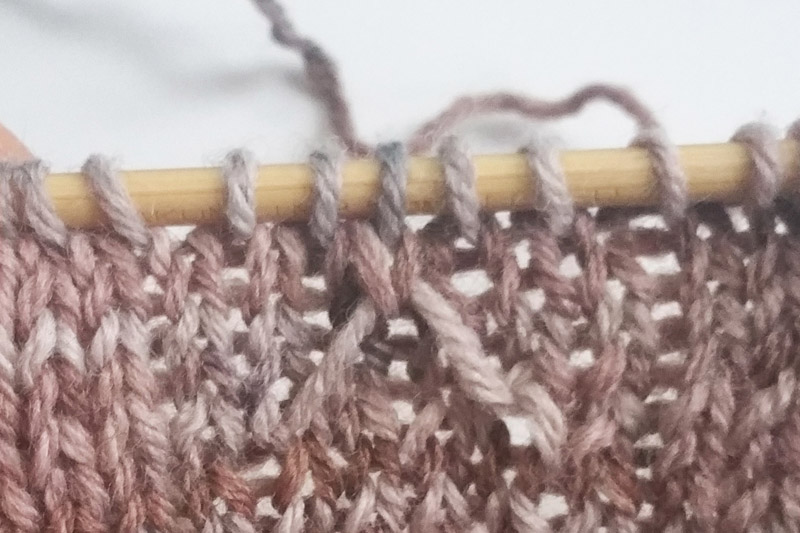
\includegraphics[height=1.5in]{end.jpg}
\end{center}

\vfill
\columnbreak
Before the \textbf{k uls}, you should have a loose strand (yellow) a few rows below the stitch you are going to work (red). The working yarn is highlighted (blue).

\begin{flushright}
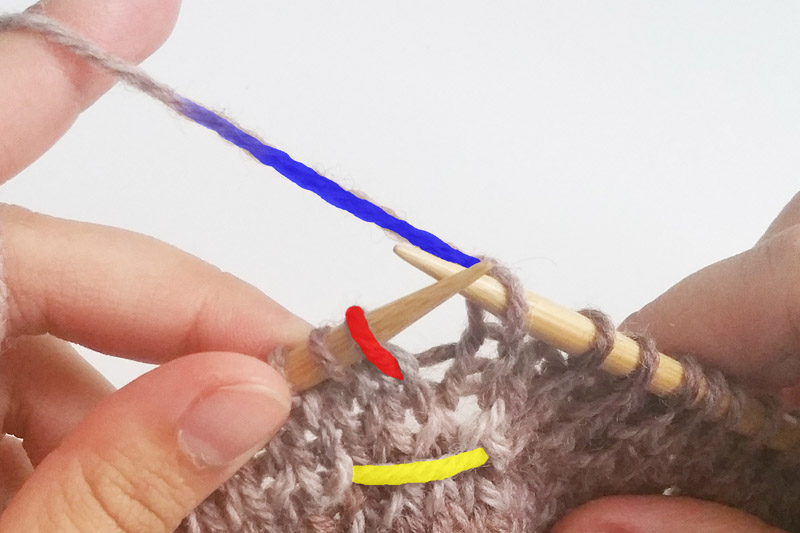
\includegraphics[height=1.5in]{setup.jpg}
\end{flushright}

\begin{enumerate}
\item Insert needle front to back underneath the loose strand.

\begin{flushright}
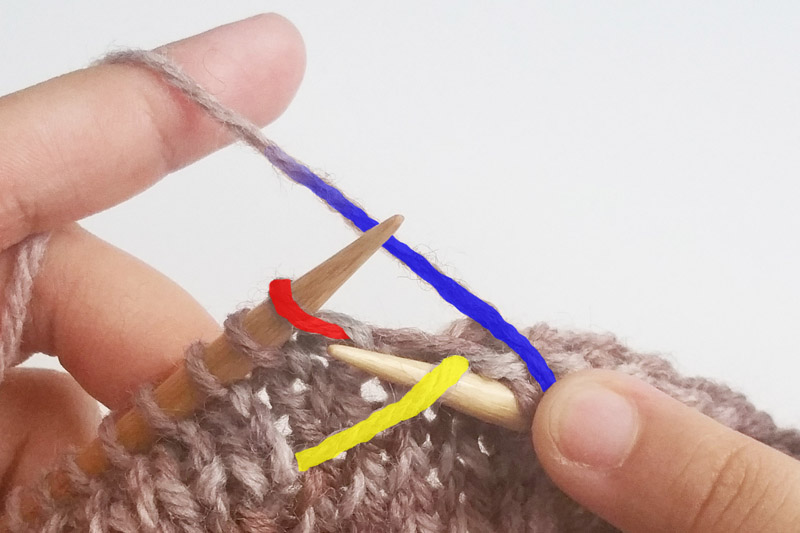
\includegraphics[height=1.5in]{step1.jpg}
\end{flushright}

\item From here, knit into the next stitch normally.

\begin{flushright}
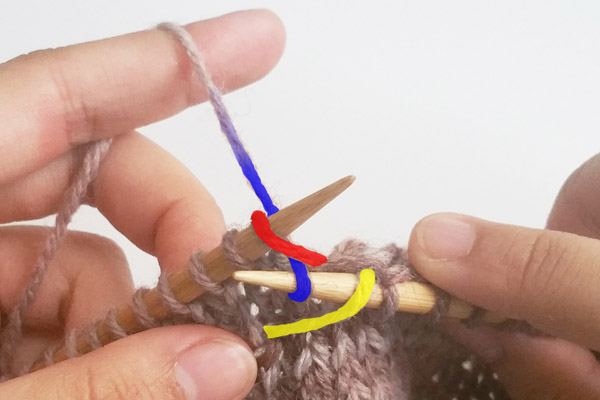
\includegraphics[height=1.5in]{step2.jpg}
\end{flushright}

\item Bring the new stitch underneath the loose strand from back to front, then pull the old stitch off the left needle.

\begin{flushright}
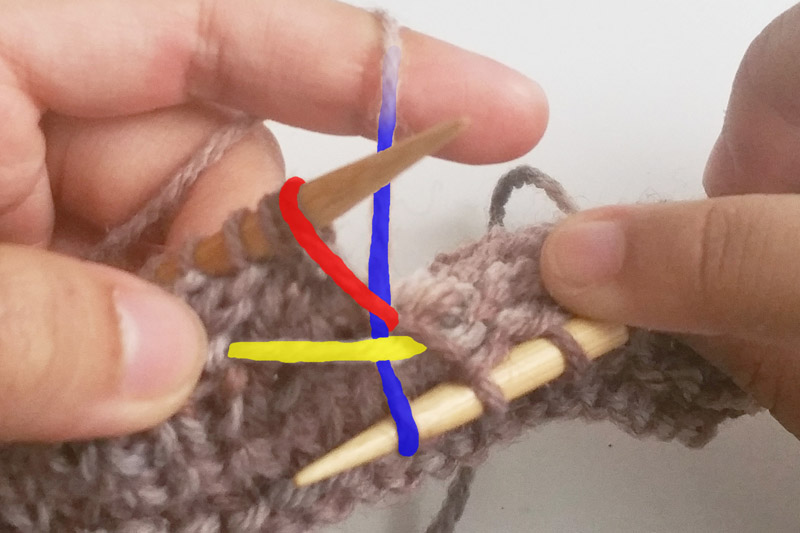
\includegraphics[height=1.5in]{step3.jpg}
\end{flushright}


\end{enumerate}

\end{multicols}

\end{document}